\documentclass[11pt, a4paper]{article}

% --- PAQUETES ---
\usepackage[utf8]{inputenc} \usepackage[T1]{fontenc} \usepackage[spanish,es-tabla]{babel} \usepackage{graphicx} \usepackage{amsmath} \usepackage{geometry} \usepackage{fancyhdr} \usepackage[sans]{raleway} \usepackage[table]{xcolor} \usepackage{booktabs} \usepackage{float} \usepackage{enumitem} \usepackage{hyperref} \hypersetup{colorlinks=true, linkcolor=blue, urlcolor=cyan}

% --- CONFIGURACIÓN ---
\geometry{a4paper, left=2.5cm, right=2.5cm, top=3cm, bottom=3cm, headheight=15pt}
\renewcommand{\familydefault}{\sfdefault} \setlength{\parindent}{0pt} \setlength{\parskip}{1.2ex}

% --- ENCABEZADO Y PIE DE PÁGINA ---
\pagestyle{fancy} \fancyhf{} \fancyhead[L]{
\includegraphics[height=1cm]{logo_wasaff_consulting.png}}
\fancyhead[R]{\itshape{Dossier de Ingeniería} \\ \textbf{Proyecto FinanSys - Resiliencia Térmica}}
\fancyfoot[C]{\thepage} \renewcommand{\headrulewidth}{0.4pt} \renewcommand{\footrulewidth}{0.4pt}

% --- PORTADA ---
\title{
    \vspace{2cm} 
\includegraphics[height=4cm]{logo_wasaff_consulting.png}\\[2cm]
    \huge{\textbf{Dossier de Ingeniería}}\\[0.5cm]
    \Large{Análisis de Respaldo Térmico para Continuidad Operacional de Data Center}\\[1.5cm]
}
\author{
    \large{Preparado para: \textbf{FinanSys (Nombre Confidencial)}}\\[2cm]
    \large{Preparado por: \textbf{Felipe Wasaff}}\\
    \large{\textit{Fundador, Wasaff Consulting}}\\[0.2cm]
    \texttt{felipe@wasaffconsulting.com}
}
\date{Octubre de 2025}

% =============================================================================
% INICIO DEL DOCUMENTO
% =============================================================================
\begin{document}

\maketitle \thispagestyle{empty} 
\newpage
\tableofcontents \thispagestyle{empty}
\newpage
\setcounter{page}{3} 

% --- SECCIÓN 1: RESUMEN EJECUTIVO ---
\section{Resumen Ejecutivo y Recomendaciones}
FinanSys enfrenta un riesgo operacional crítico: 5 minutos sin enfriamiento activo durante el restablecimiento de su chiller. Este diagnóstico cuantifica el problema, valida una solución robusta mediante simulación avanzada y propone una arquitectura costo-eficiente.

Nuestro análisis concluye:
\begin{itemize}
    \item \textbf{Carga Térmica Crítica:} Se deben absorber \textbf{148.5 Megajoules (MJ)} durante el período de riesgo para evitar una falla catastrófica.
    \item \textbf{Insuficiencia del Sistema Actual:} El tanque de 1700 litros es incapaz de manejar esta carga, alcanzando la temperatura límite en aproximadamente \textbf{76 segundos}.
    \item \textbf{La Solución no es solo Volumen:} Un tanque del tamaño correcto pero mal diseñado puede ser inútil. Nuestro análisis CFD demuestra que un diseño no optimizado puede **reducir la efectividad del respaldo en más de un 60\%** debido a cortocircuitos térmicos.
\end{itemize}

\subsection*{Recomendación Principal}
\textbf{Wasaff Consulting recomienda la implementación de una "Solución Híbrida Inteligente Optimizada por Simulación".} Esta arquitectura combina un sistema de acumulación térmica de \textbf{7,500 litros} con un diseño interno de difusores validado por CFD (Figura \ref{fig:cfd_results}), junto a un sistema de bombeo respaldado por un \textbf{UPS industrial}. Esto representa el balance óptimo entre confiabilidad, eficiencia y Costo Total de Propiedad (TCO).

% --- SECCIÓN 2: METODOLOGÍA ---
\section{Metodología de Análisis}
Se utilizó un enfoque multi-escala:
\begin{itemize}
    \item \textbf{Modelo de Sistema (0D):} Se desarrolló un modelo computacional en Python para simular el balance de energía global del sistema ($E = m \cdot c_p \cdot \Delta T$) y dimensionar el volumen de acumulación requerido.
    \item \textbf{Modelo de Componente (CFD):} Se utilizó un modelo de Dinámica de Fluidos Computacional (implementado en FEniCS) para analizar la convección natural y la estratificación térmica dentro del tanque de acumulación, optimizando el diseño para máxima eficiencia.
\end{itemize}

% --- SECCIÓN 3: RESULTADOS ---
\section{Resultados del Análisis}
\subsection{Insuficiencia del Sistema Actual}
La simulación del sistema de 1700 litros confirma su falla en proveer el respaldo necesario. La Figura \ref{fig:falla_actual} ilustra la rápida escalada de temperatura.

\begin{figure}[H]
    \centering
    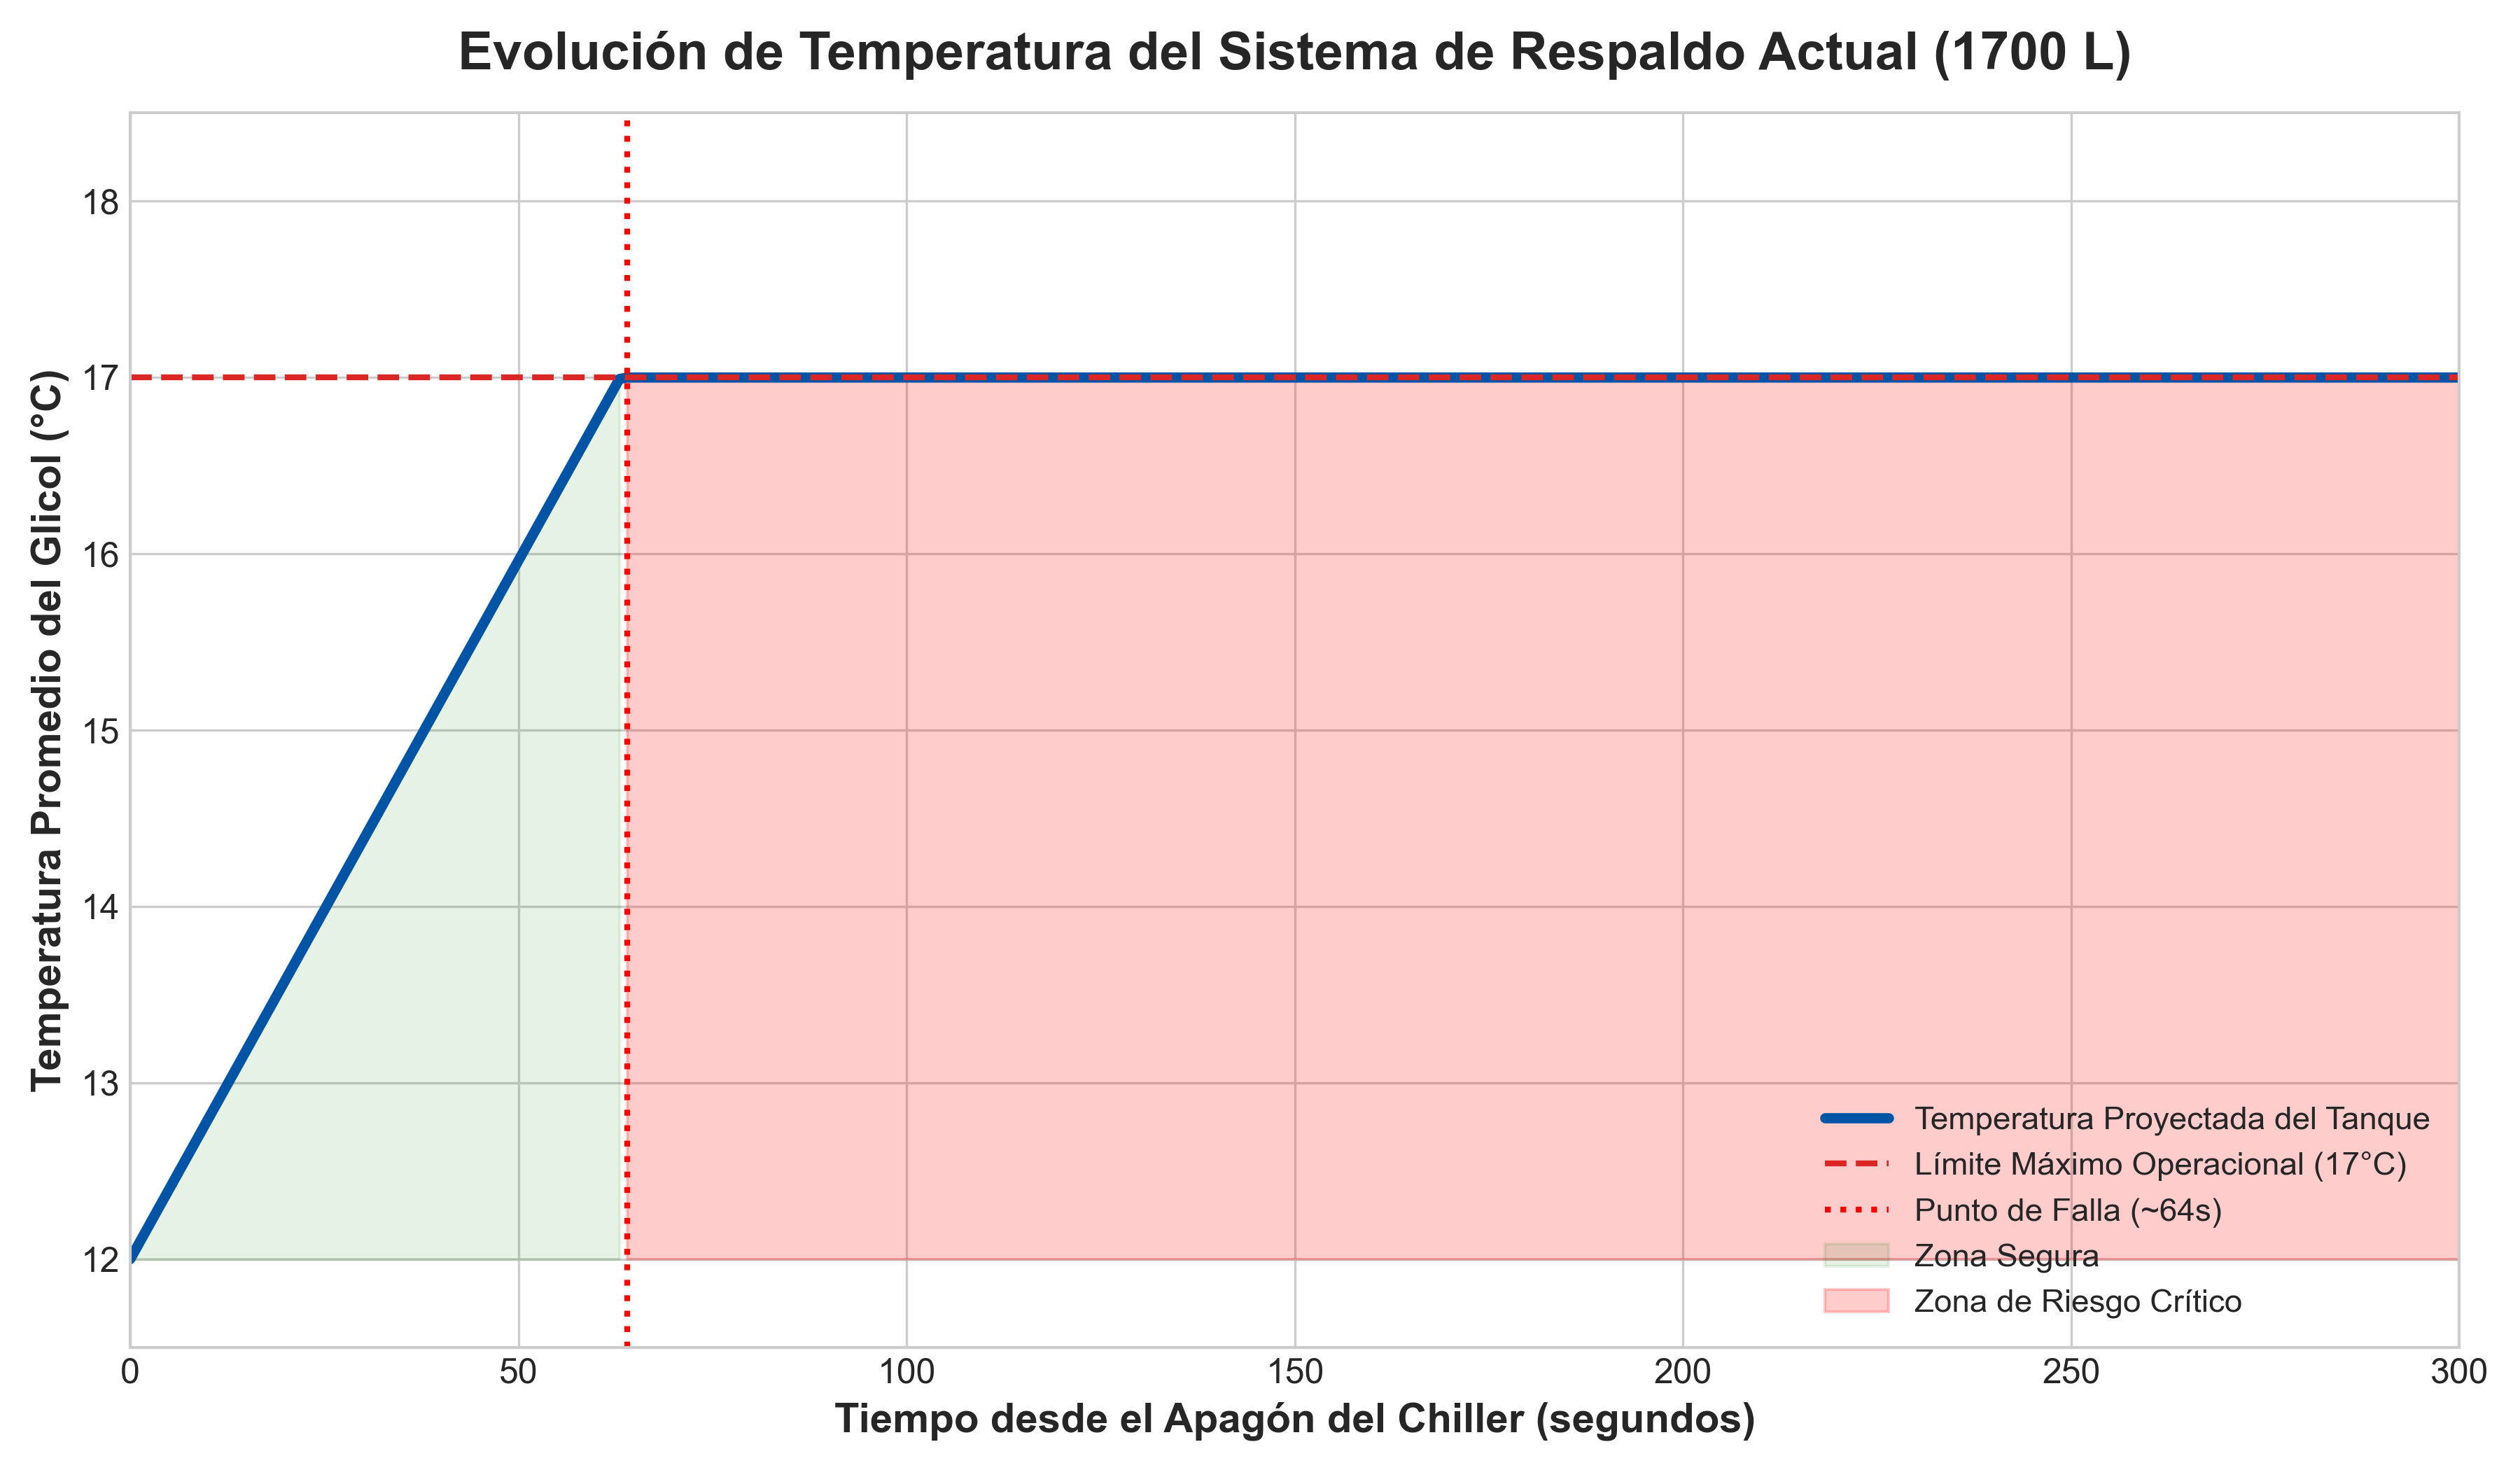
\includegraphics[width=0.9\textwidth]{grafico_falla_actual.png}
    \caption{Evolución de temperatura del sistema actual (1700 L). El límite se alcanza en $\sim$76s.}
    \label{fig:falla_actual}
\end{figure}

\subsection{Dimensionamiento y Validación CFD de la Solución Propuesta}
Se determinó que se requiere un sistema de 7,500 litros para absorber la carga térmica. Sin embargo, el volumen por sí solo no garantiza el éxito. Es crítico asegurar que la estratificación térmica dentro del tanque sea efectiva.

La Figura \ref{fig:cfd_results} compara el rendimiento de un diseño estándar vs. el diseño optimizado por Wasaff Consulting.

\begin{figure}[H]
    \centering
    \includegraphics[width=\textwidth]{simulacion_diseno_estandar.png} 
    \hspace{0.5cm} % Espacio entre imágenes
    \includegraphics[width=\textwidth]{simulacion_diseno_optimizado.png}
    \caption{Análisis CFD a los 100s. \textbf{Izquierda:} Diseño estándar mostrando cortocircuito térmico (zona azul inutilizada). \textbf{Derecha:} Diseño optimizado con difusor, logrando una estratificación efectiva y el uso de todo el volumen de acumulación.}
    \label{fig:cfd_results}
\end{figure}

El análisis CFD valida que nuestro diseño propuesto previene fallas de rendimiento y maximiza el uso del volumen térmico, garantizando la resiliencia del sistema durante los 300 segundos críticos.

\newpage
% --- SECCIÓN 4: RECOMENDACIÓN FINAL ---
\section{Recomendación: La Solución Híbrida Inteligente}
Proponemos formalmente una arquitectura que ataca el problema térmico y el hidráulico con un enfoque de optimización de costos y riesgos:

\begin{itemize}[leftmargin=*, itemsep=1.5ex]
    \item \textbf{Componente 1: Sistema de Acumulación Térmica Optimizada por CFD (7,500L).} Se instalan tanques a nivel de piso con un volumen total de 7.5 m³, incluyendo los difusores internos diseñados para garantizar la estratificación térmica y máxima eficiencia.
    \item \textbf{Componente 2: Sistema de Bombeo de Emergencia con UPS.} La bomba de recirculación se conecta a un UPS de grado industrial, asegurando el flujo constante durante más de 10 minutos con un bajo CAPEX y sin riesgo estructural.
\end{itemize}

\subsection*{Ventajas del Enfoque Wasaff Consulting}
\begin{itemize}
    \item \textbf{Optimización del Diseño (Valor CFD):} No solo dimensionamos el tanque, sino que garantizamos su correcto funcionamiento, eliminando el riesgo de que la inversión sea inútil por un mal diseño hidráulico.
    \item \textbf{Reducción del TCO (Costo Total de Propiedad):} La solución híbrida (tanque en piso + UPS) presenta el menor costo de ciclo de vida al minimizar el CAPEX de obras civiles y el OPEX de operación.
    \item \textbf{Seguridad y Confiabilidad:} El diseño es inherentemente más seguro y robusto que alternativas como la elevación de grandes masas.
\end{itemize}

% --- SECCIÓN 5: CONCLUSIÓN ---
\section{Conclusión y Próximos Pasos}
Wasaff Consulting ha transformado un problema de riesgo en una solución de ingeniería validada por simulación avanzada. La ``Solución Híbrida Inteligente'' es la opción más robusta, segura y rentable.

Recomendamos avanzar a una fase de \textbf{Ingeniería de Detalle} para construir los planos de fabricación de los tanques y difusores, especificar los componentes y desarrollar la lógica de control.

% --- NOTA FINAL ---
\vspace{1.5cm}
\begin{center}
\rule{0.8\textwidth}{0.4pt} \vspace{0.3cm}
\parbox{0.8\textwidth}{\footnotesize\itshape \textbf{Nota Importante sobre el Alcance:} Este documento constituye el Diagnóstico Estratégico. Wasaff Consulting está preparado para entregar una propuesta comercial detallada para la fase subsecuente de "Ingeniería de Detalle".}
\end{center}

\end{document}